\documentclass{resume}
\usepackage[left=0.6in,top=0.6in,right=0.6in,bottom=0.6in]{geometry}
\usepackage[svgnames]{xcolor}
\usepackage{hyperref}
\hypersetup{
  colorlinks=true,
  allcolors=DarkRed,
  pdfborderstyle={/S/U/W 1}
}

\usepackage{vwcol}
\usepackage{natbib}
\usepackage{cfr-lm}
\usepackage{graphicx}
\usepackage{enumitem}

\begin{document}

%%%%%%%%%%%%%%%%%%%%%%%%%%%%%%%%%%%%%%%%%%%%%%%% TITLE SECTION
\vspace{-2em}
\begin{minipage}{0.75\textwidth}
    \raggedright
    {\Huge \textbf{Carolina Brañas}}\\[0.5em] 
    {\small
    (+34)$\cdot$644$\cdot$004$\cdot$477 \\
    \href{mailto://carobrasor@gmail.com}{carobrasor@gmail.com} \\
    \href{https://carobs9.github.io/}{carobs9.github.io} \\
    \href{https://github.com/carobs9}{github.com/carobs9} \\
    \href{https://www.linkedin.com/in/carolinabranas/}{linkedin.com/in/carolinabranas} \\
    Madrid, Spain
    }\\[1em]
    %{\normalsize \textbf{Data Scientist}}\\[0.5em]
    % {\LARGE \textbf{Data Scientist}}\\[0.5em]
    I am a data scientist, passionate about machine learning, network analysis, natural language processing, and geospatial data. \\
    I have a keen interest in data visualization and its role in communicating insights effectively.
\end{minipage}%
\hfill
\begin{minipage}{0.23\textwidth}
    \begin{flushright}
        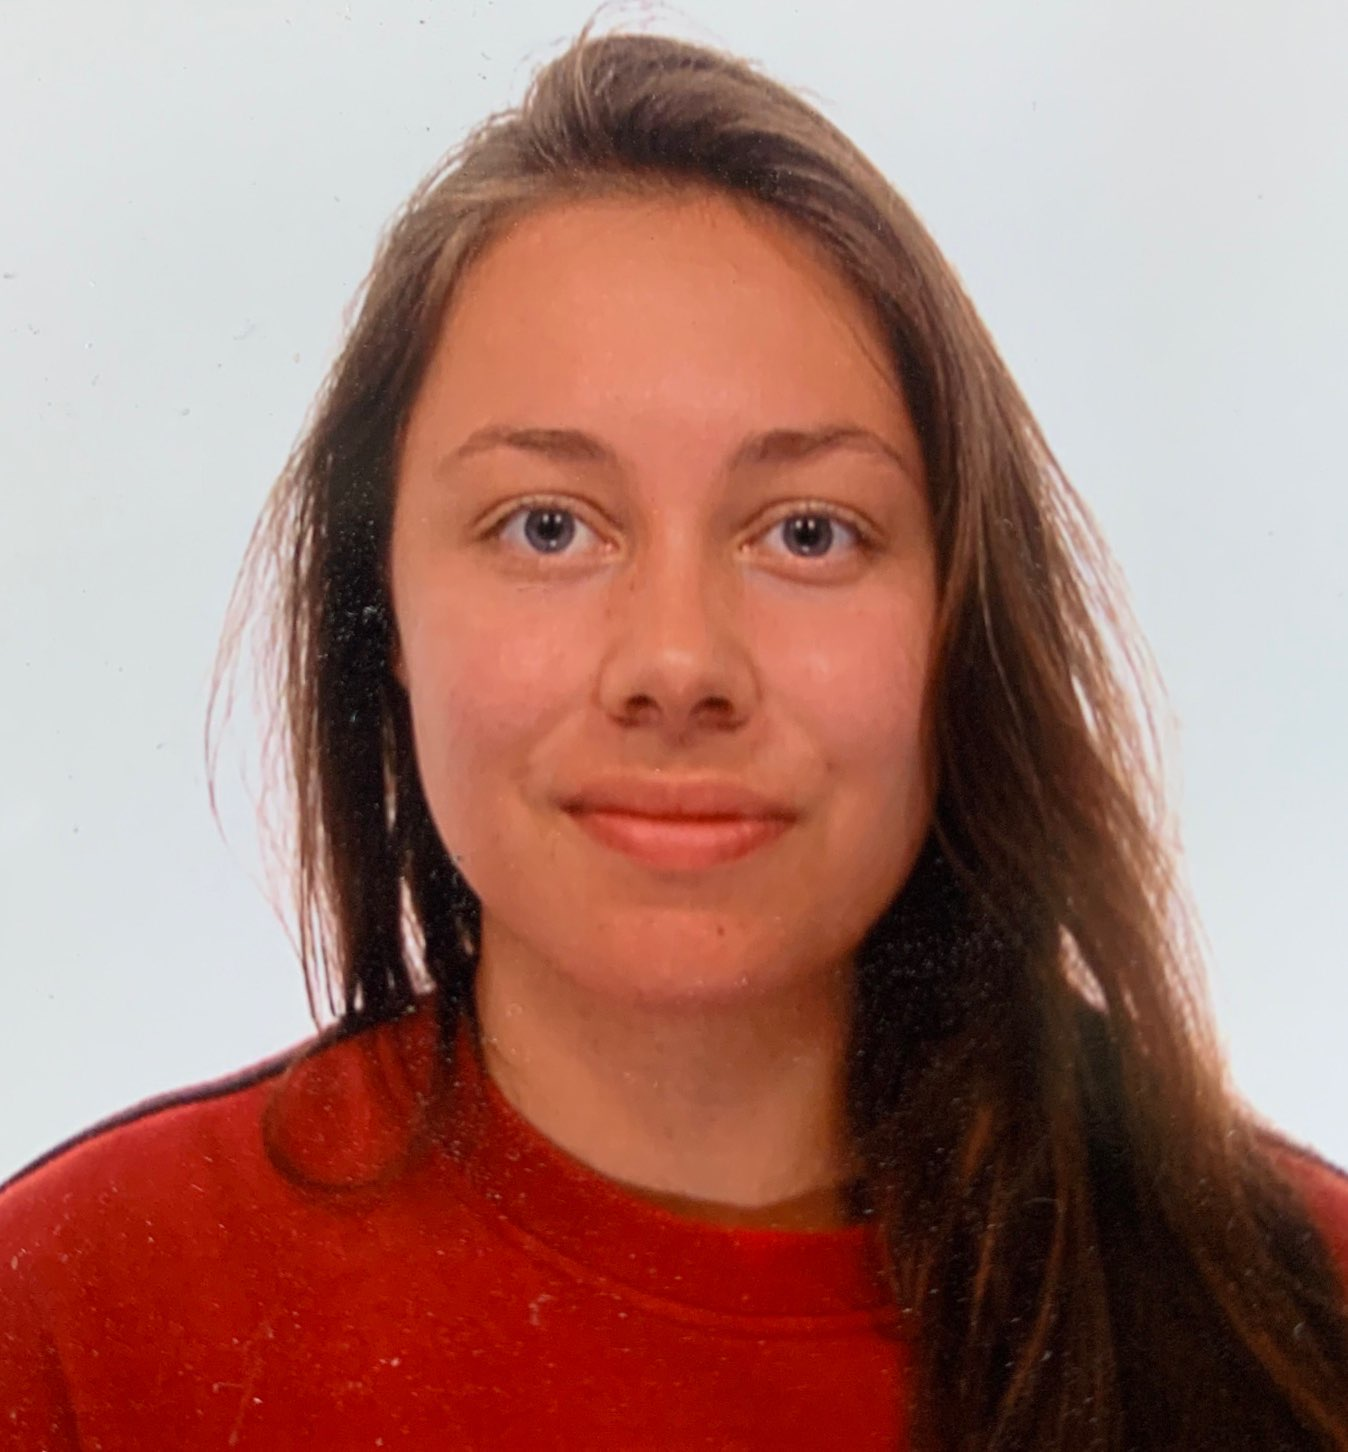
\includegraphics[width=3cm]{profile.jpg}
    \end{flushright}
\end{minipage}
\vspace{1em}

%%%%%%%%%%%%%%%%%%%%%%%%%%%%%%%%%%%%%%%%%%%%%%%% RESEARCH EXPERIENCE
\section{EXPERIENCE}
\begin{content}

    \begin{position}{Research Assistant, Data Science}{May 2024 -- present}{University of Copenhagen}{Prof.~Jeanet Bentzen}{}
    \item Contributed to the {\href{https://www.economics.ku.dk/research/externally-funded-research_new/shocking-religion/}{Shocking Religion}} project, analyzing economic effects of religious shocks.
    \item Constructed and deployed topic modeling solutions with SentenceTransformers and BERTopic; developed LLM-based pipelines using retrieval-augmented generation (RAG) for contextual document analysis.
    \item Conducted time series analysis and built visualizations to interpret long-term socioeconomic patterns.
    \item Presented findings through technical reports and presentations tailored to diverse audiences.
    \item Designed, dockerized, and deployed data solutions; leveraged UCloud to streamline large-scale data processing.
    \end{position}

    \begin{position}{Data Scientist}{October 2023 -- May 2024}{Above Sports}{}{}
    \item Built computer vision models to improve company’s logo detection tool.
    \item Collaborated on process automation and product performance enhancements.
    \end{position}

    \begin{position}{Marketing Strategist}{September 2021 -- May 2022}{Crescendo Collective}{}{}
    \item Conducted data analysis using Google Analytics and Ads, delivering actionable insights.
    \item Led market research and supported automation of internal analytics pipelines.
    \end{position}

\sectionlineskip
\end{content}

%%%%%%%%%%%%%%%%%%%%%%%%%%%%%%%%%%%%%%%%%%%%%%%% EDUCATION 
\section{EDUCATION} 
\begin{content}
    {\bf M.Sc. Social Data Science} \hfill {\bf 2022 -- 2024} \\
    University of Copenhagen \\
    {\em Thesis:} {\href{https://carobs9.github.io/segregation-mobility/}{Mobility and income segregation in Madrid, Spain}} \\
    {\em Elective Courses:}
    \begin{itemize}[noitemsep, topsep=0pt, leftmargin=*]
        \item Advanced Machine Learning for Data Science (IT University of Copenhagen)
        \item Geospatial Data Science (IT University of Copenhagen)
        \item Advanced Network Science (IT University of Copenhagen)
        \item Natural Language Processing (Department of Computer Science, DIKU)
    \end{itemize}

    \medskip

    {\bf B.Sc. Marketing} \hfill {\bf 2018 -- 2022} \\
    Cardinal Stritch University \\
    {\em Dean's List (2018--2022)} \\
    {\em Best Graduating GPA in Marketing B.Sc. (2022)}

    {\bf Computer Science Minor} \hfill {\bf 2018 -- 2022} \\
    Cardinal Stritch University \\
\sectionlineskip
\end{content}

%%%%%%%%%%%%%%%%%%%%%%%%%%%%%%%%%%%%%%%%%%%%%%%%% LANGUAGES
\section{LANGUAGES} 
\begin{content}
    {\bf Spanish and Galician:} Native \\
    {\bf English:} Professional Proficiency  \\
    {\bf Portuguese:} Beginner \\
\end{content}

%%%%%%%%%%%%%%%%%%%%%%%%%%%%%%%%%%%%%%%%%%%%%%%%% AWARDS
\section{AWARDS}
\begin{content}
    \prize{Dean's List}{2018--2022}{Achieved Dean’s List every semester of B.Sc. for a GPA above 3.5 with at least 12 credits.}

    \prize{Best Graduating GPA of Marketing B.Sc.}{2022}{Graduated with the top GPA (3.8/4.0) in Marketing.}

    \prize{Academic and Athletic Grant}{2018--2022}{Received a full scholarship for academic excellence and soccer performance over four years.}
\end{content}

%%%%%%%%%%%%%%%%%%%%%%%%%%%%%%%%%%%%%%%%%%%%%%%%% PROJECTS
\section{PROJECTS \textbf{\em\&} EXTRACURRICULARS} 
\begin{content}

    \begin{position}{Mobility and Income Segregation in Madrid}{2023}{\href{https://github.com/carobs9/segregation-madrid}{segregation-madrid}}{Master's Thesis project}{}
    \item Analyzed mobility and income segregation patterns using geospatial data, network analysis, and visual storytelling in Python.
    \end{position}

   %\begin{position}{LLM PDF Retrieval (RAG)}{2024}{\href{https://github.com/carobs9/llm-pdf-retrieval}{github.com/carobs9/llm-pdf-retrieval}}{}{Personal}
   %\item Built a retrieval-augmented generation (RAG) pipeline using LLMs to answer questions from PDFs. Focused on preprocessing, chunking, embedding, and vector search.
   %\end{position}

    \begin{position}{CycleGAN Monet}{2023}{\href{https://github.com/carobs9/CycleGAN_Monet}{CycleGAN\_Monet}}{Academic project for Advanced Machine Learning course}{}
    \item Trained a CycleGAN model to convert real photos into Monet-style images. Implemented with PyTorch and conducted visual evaluation of stylization results.
    \end{position}
    
\sectionlineskip    
\end{content}

%%%%%%%%%%%%%%%%%%%%%%%%%%%%%%%%%%%%%%%%%%%%%%%%% TECHNICAL SKILLS
\section{SKILLS} 
\begin{content}
    {\bf PROGRAMMING:} Python {\footnotesize (numpy, tensorflow, matplotlib, pytorch)}, SQL, Bash \\
    {\bf ML \& NLP:} Transformers, Topic Modeling {\footnotesize (umap, hdbscan, bertopic)}, Scikit-learn, Hugging Face \\
    {\bf GEOSPATIAL:} Geopandas, Rasterio, QGIS \\
    {\bf CLOUD / TOOLS:} UCloud, Git, Docker, Linux, VSCode
\end{content}

\end{document}
